%%%%%%%%%%%%%%%%%%%%%%%%%%%%%%%%%%%%%%%%%
% University Assignment Title Page 
% LaTeX Template
% Version 1.0 (27/12/12)
%
% This template has been downloaded from:
% http://www.LaTeXTemplates.com
%
% Original author:
% WikiBooks (http://en.wikibooks.org/wiki/LaTeX/Title_Creation)
%
% License:
% CC BY-NC-SA 3.0 (http://creativecommons.org/licenses/by-nc-sa/3.0/)
% 
% Instructions for using this template:
% This title page is capable of being compiled as is. This is not useful for 
% including it in another document. To do this, you have two options: 
%
% 1) Copy/paste everything between \begin{document} and \end{document} 
% starting at \begin{titlepage} and paste this into another LaTeX file where you 
% want your title page.
% OR
% 2) Remove everything outside the \begin{titlepage} and \end{titlepage} and 
% move this file to the same directory as the LaTeX file you wish to add it to. 
% Then add \input{./title_page_1.tex} to your LaTeX file where you want your
% title page.
%
%%%%%%%%%%%%%%%%%%%%%%%%%%%%%%%%%%%%%%%%%
%\title{Title page with logo}
%----------------------------------------------------------------------------------------
%	PACKAGES AND OTHER DOCUMENT CONFIGURATIONS
%----------------------------------------------------------------------------------------

\documentclass[11pt]{article}
\usepackage[english]{babel}
\usepackage[utf8x]{inputenc}
\usepackage{amsmath}
\usepackage{fancyhdr}
\usepackage{graphicx}
\usepackage[colorinlistoftodos]{todonotes}
\usepackage{geometry}
\pagestyle{fancy}
\geometry
{
 a4paper,==
 total={170mm,257mm},
 left=20mm,
 top=20mm,
}
\fancyheadoffset{0.1cm}
\lhead{Mingyang Zhang : 650242, Shreyash Patodia : 767336}
\rhead{mingyang, spatodia}



\begin{document}

\section{Introduction}

DISTANCE MEASURE AND VOTING METHOD FOR EVERYTHING AND DATASET IN QUESTION. (Use all metrics for all things). 

In this assignment we were asked to classify instances in the Abalone Dataset into one of two 
('young' or 'old') or three ('very young', 'old' and 'middle-age') categories. The classification method meant to be used was K-Nearest Neighbours. 


\section{Similarity Metrics}

\subsection{Euclidean Distance, Manhattan Distance and Minkowski Distance}

The Abalone data set contains eight attributes out of which 7 are of a continuous nature, so it made sense to us to use some sort of distance metric to evaluate similarity instead of checking for equality (like in the case for Jaccard and Dice Similarity) or doing something like cosine similarity (which would compare the angles between the abalones since two abalones can be very similar in proportions, and thus have small angle and high cosine similarity but one may be much larger and older than the other). If p and q are the instances to be compared the formula for our similarity metrics are: \\

Euclidean Distance:
\begin{equation}
\sqrt{\sum_{i=1}^{n} (p_{i} - q_{i})^{2}}
\end{equation}

Manhattan Distance:
\begin{equation}
\sum_{i=1}^{n} |p_{i} - q_{i}|
\end{equation}

Minkowski Distance:
\begin{equation}
{(\sum_{i=1}^{n} {|p_{i} - q_{i}|}^{pow})}^{1/pow}
\end{equation}

(We take pow = 0.5 for Minkowski distance, as it lets us makes for a nice comparison with Euclidean since Euclidean is basically Minkowski with p = 2) \\

Euclidean takes sum of squares before finding the root, Manhattan is plain addition of distances values and Minkowski (with p = 0.5) takes the root of each value before summing them up and squaring the sum. We especially wanted to contrast Minkowski and Euclidean since Minkowski is actually going to amplify larger distances (since most distances are < 1 and root of a number with value < 1 will be large than the number itself) and Euclidean would tend to supress it by squaring (square of number < 1 is less than the number itself). 


\subsection{Experimentation with similarity metrics}

Here are some results we got from testing our similarity metrics while varying other parameters in the program. 
The experiment shows us that that the performance of all of the similarity metrics is very closely lumped together, this is probably due to the fact that the distances are so small that it doesn't make much of a difference if we square or find the root of the values. 

(Note: All measurements in the tables are averages of 10 runs and 10 fold cross validation was used for each run)
\begin{table}
\centering
\begin{tabular}{|p{2cm}|p{3cm}||p{2cm}|p{1.5cm}|p{1.5cm}|p{1.5cm}|}
 \hline
 \multicolumn{6}{|c|}{Similarity Experiment} \\
 \hline
 Classification Type & Parameters & Similarity Metric & Accuracy & Precision & Recall\\
 \hline
 Abalone-3 & k=29,voting=inv. distance &   euclidean & 0.7676  & 0.6469 & 0.6487\\
 \hline
 Abalone-3 & k=29,voting=inv. distance &   minkowski & 0.7663 & 0.6468 & 0.6473\\
 \hline
 Abalone-3 & k=29,voting=inv. distance &   manhattan & 0.7641 & 0.6420 & 0.6436\\ 
 \hline
 \hline
 Abalone-2 & k=29,voting=inv. distance &   euclidean & 0.7857  & 0.7714 & 0.7399\\
 \hline
 Abalone-2 & k=29,voting=inv. distance &   minkowski & 0.7787 & 0.7654 & 0.7299\\
 \hline
 Abalone-2 & k=29,voting=inv. distance &   manhattan & 0.7830  & 0.7683 & 0.7355\\ 
 \hline

\end{tabular}
\caption{Table of experiments with different similarity metric}
\end{table}
\label{Figure 1}


% Commands to include a figure:
%\begin{figure}[!htb]
%\centering
% \includegraphics[width=0.5\textwidth]{BadExample.png}
% \caption{\label{fig:frog}Bad Design Example}
%\end{figure}


\section{Validation Framework}

\subsection{M-Fold Cross Validation}

For our validation framework we used 10-Fold Cross Validation, we first divide the dataset into 10 (approximately) equal partitions and then perform K-Nearest Neighbour classification by choosing each of the 10 partitions as our test set (and the amalgamation of the remaining 9 as our training set) for one run of the K-Nearest Neighbour algorithm. This leads to very stable evaluation metrics across different runs of the program since performing the algorithm 10 times means that any positive outlier is (very likely to be) averaged out by negative ones
. In our strategy, if the data set cannot be divided into partitions of equal sizes then we just keep on adding one instance to the partitions (starting at the 0th partition) until there are no instances remaining.\\

We also tested 10-Fold Cross Validation with holdout (split at 90:10), 5-Fold Cross Validation and 20-Fold Cross Validation and here is a graph of their accuracies for 10 different runs with abalone-2 and abalone-3 each:


% Commands to include a figure:
%\begin{figure}[!htb]
%\centering
% \includegraphics[width=0.5\textwidth]{BadExample.png}
% \caption{\label{fig:frog}Bad Design Example}
%\end{figure}

\begin{figure}[!htb]
\centering

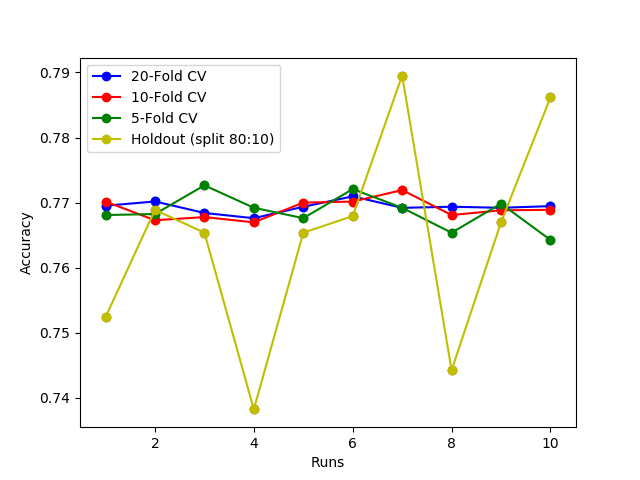
\includegraphics[width=0.5\textwidth]{consistency_comparison_3.png}
\caption{Comparison of consistency for different validation methods with Abalone-3}
\end{figure}

\begin{figure}[!htb]
\centering

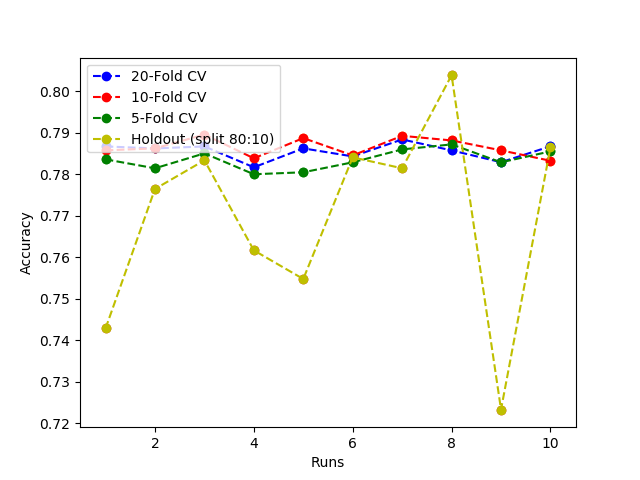
\includegraphics[width=0.5\textwidth]{consistency_comparison_2.png}
\caption{Comparison of consistency for different validation methods with Abalone-2}
\end{figure}

\\ 

From the above graphs it is clear that cross-validation is far more consistent in terms of predictive accuracy than holdout. 



\section{Our choices}

\subsection{Representation of Data}

We are using a 2-tuple to represent the data set wherein the first element of the tuple is the list of instances and the second element of the data set is the list of class labels corresponding to the instances. \\
In our pre-processing of the data we determined that it was best to work with all of the attributes other than the Gender. We chose to remove gender from the reckoning because in order to use gender in our similarity metrics we had to do some sort of numerical transformation which was not guaranteed to be ideal. Moreover, our tests without gender being turned into -1, 0, 1 for Male, Infant and Female respectively show higher (but comparable) accuracy and comparable precision and recall to when gender was turned into an ordered value for similarity comparison, meaning that it was in the best interest of efficiency to get rid of gender.  \\
We also found that height and shucked weight are very low for abalones with label "very-young" and is quite a bit higher for older abalones, so we decided to scale these two attributes by a factor of 2 to make this difference more pronounced. 

\subsection{A good similarity metric}

Since in our considerations of the abalone data set we are only looking at continuous data (removing the gender attribute altogether), and even if we did consider gender turning it into some sort of number representation would probably be desired. We also want to be able to approximate the age of the abalone (more rings ~ older), We know that the abalones with similar weight, height, diameter will probably fall into similar age categories. Something like Jaccard or Dice Similarity would only check for equality and would not fit in well here since we are dealing with numbers. Moreover, cosine similarity would give a small angle (high similarity) even if two items were of vastly different sizes if they had similar proportions. So we chose to use Euclidean, Minkowski and Manhattan Distance all of which would try to measure difference in the attributes of instances and we believe any of these three would be a fair choice for this dataset. For the sort of representation we use Euclidean Distance seems to be the best choice as it gives us higher accuracy, precision and recall consistently as seen in Table 1. 

\subsection{A good value of k}

In order to find a good value of k what we did was vary k with different prime numbers between 


\end{document}